\documentclass[11pt]{article}
\usepackage[a4paper,top=0.6cm,bottom=3.0cm,left=1.9cm,right=1.9cm,footskip=2.0cm]{geometry}
\usepackage{graphicx}
\usepackage[table]{xcolor}
\usepackage{ragged2e}
\usepackage{fancyhdr}
\usepackage{fontspec}
\setmainfont{Tiro Devanagari Hindi}
\setsansfont{Tiro Devanagari Hindi}
\newfontfamily\latinfont{Carlito}
\renewcommand{\familydefault}{\sfdefault}
\definecolor{titleblue}{HTML}{0F2F4A}
\definecolor{textblack}{HTML}{1A1A1A}
\definecolor{rule}{HTML}{C9C4C0}
\definecolor{muted}{HTML}{6B635E}
\setlength{\parindent}{0pt}\setlength{\parskip}{0.5em}

\setlength{\headheight}{28pt}\setlength{\headsep}{6pt}
\newcommand{\idmfooter}{%
  \begin{minipage}{\textwidth}
    {\color{rule}\hrule height 0.7pt}\vspace{4pt}
    \noindent
    \begin{minipage}[c]{0.66\textwidth}{\scriptsize\color{muted}{\latinfont Developed by the Water and Climate Lab, IIT Gandhinagar, using hydro-meteorological data from partner agencies}.}\end{minipage}\hfill
    \begin{minipage}[c]{0.32\textwidth}\raggedleft
      
\includegraphics[height=0.62cm]{wcl.png}\hspace{6pt}%
      
\includegraphics[height=0.62cm]{iitgn.png}
    \end{minipage}\\[3pt]
    {\scriptsize\color{muted}© {\latinfont 2026 Water and Climate Lab} · {\latinfont Indian Institute of Technology Gandhinagar} · {\latinfont For research and demonstration purposes}.}
  \end{minipage}%
}
\newcommand{\idmrunhead}{%
  \begin{minipage}{\textwidth}
    {\small\bfseries\color{titleblue}{\latinfont National Drought Summary}}\hfill{\small\color{muted}{\latinfont Week ending May 20, 2026}}\\[2pt]
    {\color{rule}\hrule height 0.6pt}
  \end{minipage}%
}
\fancypagestyle{idmfoot}{\fancyhf{}\renewcommand{\headrulewidth}{0pt}\renewcommand{\footrulewidth}{0pt}\fancyfoot[C]{\idmfooter}}
\fancypagestyle{idmrun}{\fancyhf{}\renewcommand{\headrulewidth}{0pt}\renewcommand{\footrulewidth}{0pt}\fancyhead[C]{\idmrunhead}\fancyfoot[C]{\idmfooter}}
\pagestyle{idmrun}

\begin{document}

\thispagestyle{idmfoot}
\noindent
\begin{minipage}[c]{0.16\textwidth}
\includegraphics[width=\linewidth]{wcl.png}\end{minipage}\hfill
\begin{minipage}[c]{0.80\textwidth}\raggedleft
  {\fontsize{19}{22}\selectfont\bfseries\color{titleblue}{\latinfont National Drought Summary}}\\[2pt]
  {\normalsize\color{muted}{\latinfont Week ending May 20, 2026}}
\end{minipage}
\vspace{6pt}{\color{rule}\hrule height 1pt}\vspace{10pt}
\begin{center}
  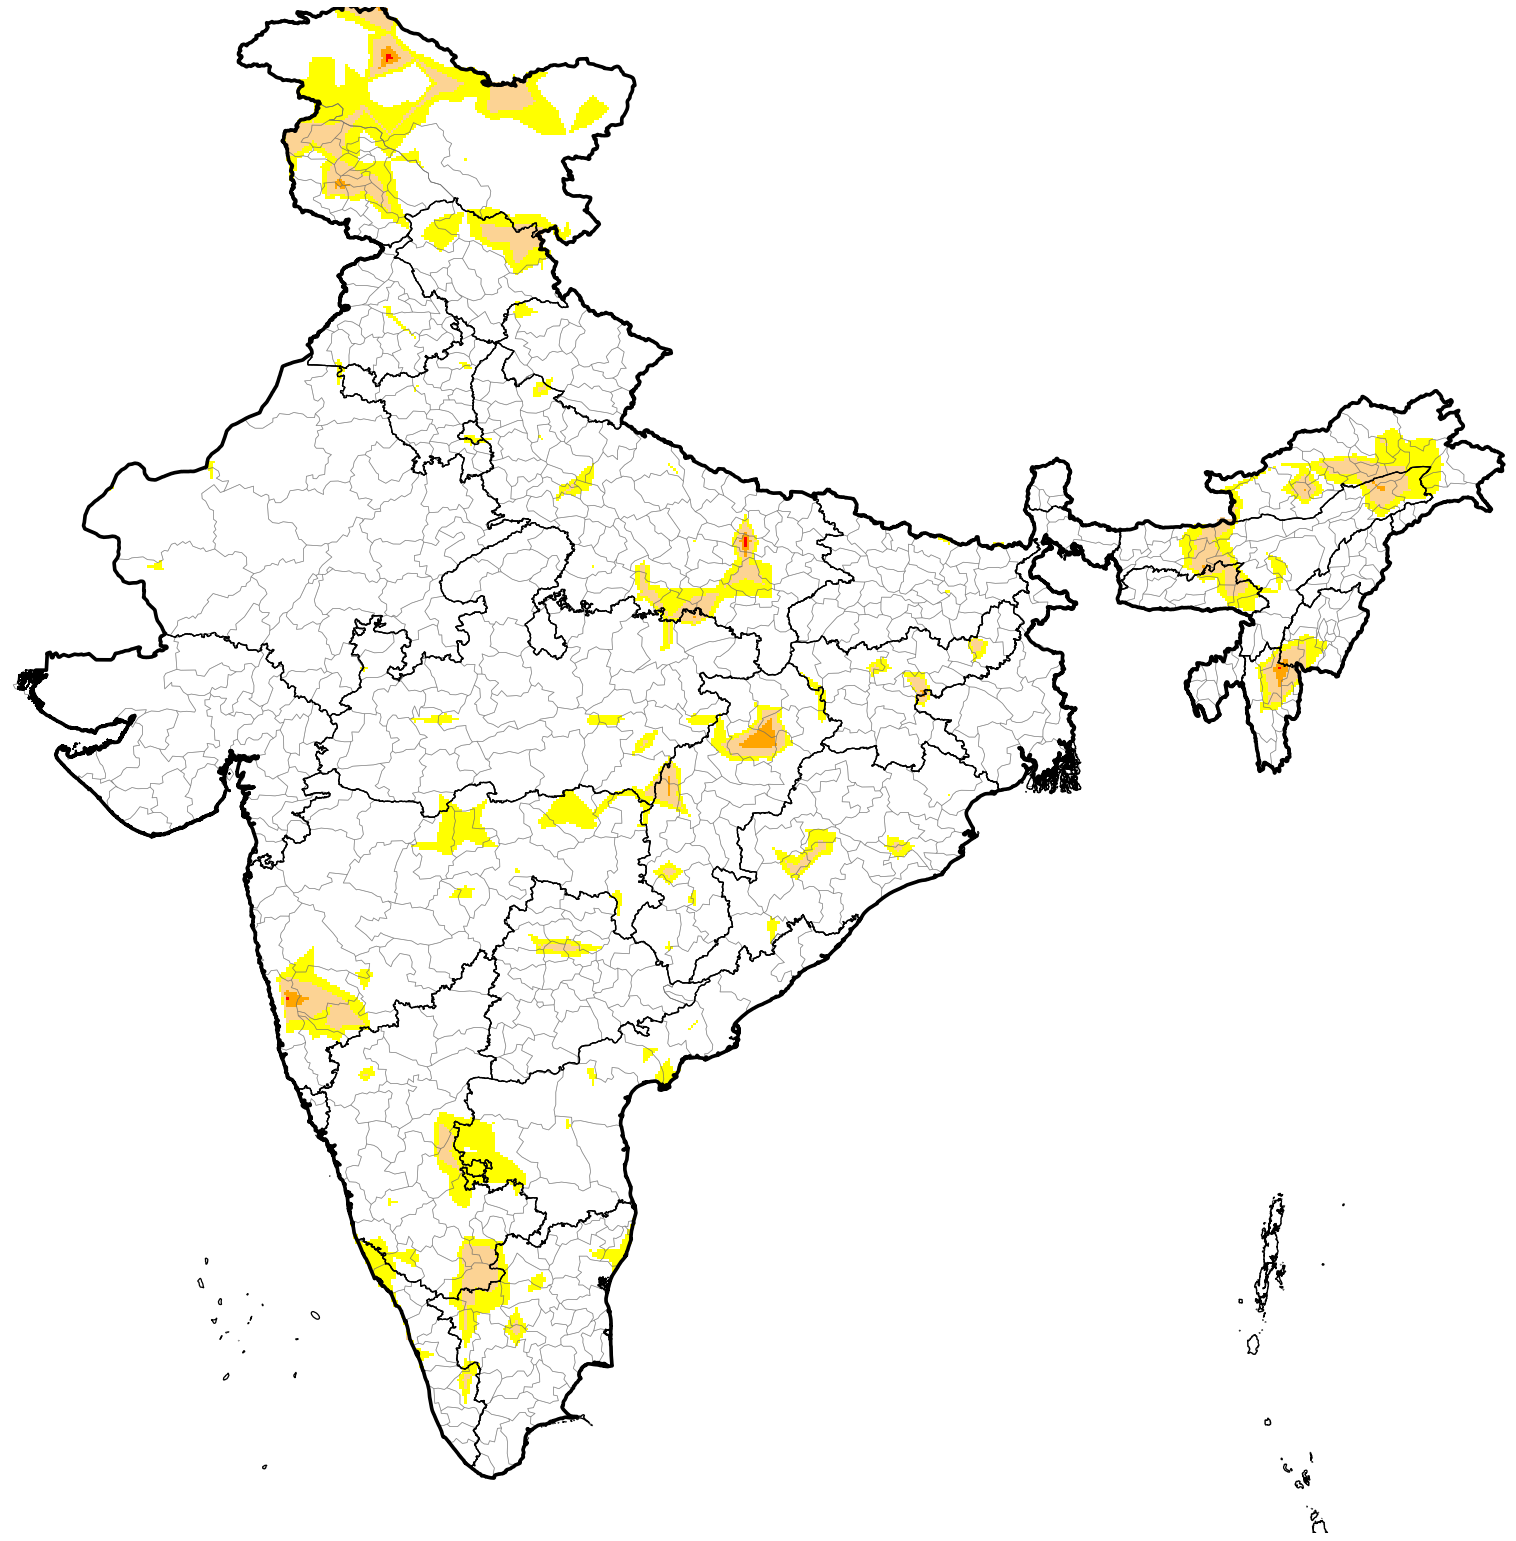
\includegraphics[width=0.60\textwidth]{cdi_map.png}\\[3pt]
  {\small\color{muted}{\latinfont Combined Drought Index (CDI) for the week ending May 20, 2026}.}
\end{center}
\vspace{2pt}
{\large\bfseries\color{titleblue}{\latinfont Summary}}\\[3pt]
{\justifying\normalsize\color{textblack}इस हफ्ता राष्ट्रीय सूखा स्थिति सामान्य श्रेणी में बड़े क्षेत्र के बने रहने से चिह्नित है, जिसमें कम हिस्सा सूखे की स्थिति का अनुभव कर रहा है। इस सप्ताह सूखा प्रभावित कुल क्षेत्र, विशेष रूप से डी{\latinfont 0} और उससे ऊपर, {\latinfont 15.3}\% था। यह पिछले सप्ताह के {\latinfont 16.2}\% की तुलना में सूखे क्षेत्र में संकुचन दर्शाता है। एक महीने पहले यह क्षेत्र लगभग {\latinfont 17.2}\% था, जो सप्ताह दर सप्ताह {\latinfont 0.9} प्रतिशत अंक का संकुचन दर्शाता है। सूखे के किसी भी वर्ग में सबसे अधिक प्रभावित राज्य दिल्ली का केंद्र शासित प्रदेश, अरुणाचल प्रदेश, जम्मू और कश्मीर, मणिपुर, मिजोरम और मेघालय थे। इसके विपरीत, सिक्किम, नागालैंड, त्रिपुरा और पश्चिम बंगाल सबसे कम प्रभावित राज्यों में थे, जिनमें सूखा {\latinfont 0.0}\% था।\par}
\vspace{8pt}
{\large\bfseries\color{titleblue}{\latinfont Regional Outlook}}\\[2pt]
{\normalsize\color{titleblue}\textbf{{\latinfont North}}}\enspace {\normalsize\color{textblack}{\latinfont Moderate, scattered drought. About 28}\% {\latinfont of the area is in drought (D0}–{\latinfont D4)}.} \par\smallskip {\normalsize\color{titleblue}\textbf{{\latinfont Northwest}}}\enspace {\normalsize\color{textblack}{\latinfont Largely normal conditions. About 4}\% {\latinfont of the area is in drought (D0}–{\latinfont D4)}.} \par\smallskip {\normalsize\color{titleblue}\textbf{{\latinfont Northeast}}}\enspace {\normalsize\color{textblack}{\latinfont Moderate, scattered drought. About 27}\% {\latinfont of the area is in drought (D0}–{\latinfont D4). Pockets of severe-or-worse conditions are present}.} \par\smallskip {\normalsize\color{titleblue}\textbf{{\latinfont East}}}\enspace {\normalsize\color{textblack}{\latinfont Mostly normal, with localised dryness. About 7}\% {\latinfont of the area is in drought (D0}–{\latinfont D4)}.} \par\smallskip {\normalsize\color{titleblue}\textbf{{\latinfont Central}}}\enspace {\normalsize\color{textblack}{\latinfont Mostly normal, with localised dryness. About 15}\% {\latinfont of the area is in drought (D0}–{\latinfont D4). Pockets of severe-or-worse conditions are present}.} \par\smallskip {\normalsize\color{titleblue}\textbf{{\latinfont West}}}\enspace {\normalsize\color{textblack}{\latinfont Moderate, scattered drought. About 22}\% {\latinfont of the area is in drought (D0}–{\latinfont D4)}.} \par\smallskip {\normalsize\color{titleblue}\textbf{{\latinfont South}}}\enspace {\normalsize\color{textblack}{\latinfont Mostly normal, with localised dryness. About 16}\% {\latinfont of the area is in drought (D0}–{\latinfont D4)}.}
\end{document}
